% Plantilla para un Trabajo Fin de Grado de la Universidad de Granada,
% adaptada para el Doble Grado en Ingeniería Informática y Matemáticas.
%
%  Autor: Mario Román.
%  Licencia: GNU GPLv2.
%
% Esta plantilla es una adaptación al castellano de la plantilla
% classicthesis de André Miede, que puede obtenerse en:
%  https://ctan.org/tex-archive/macros/latex/contrib/classicthesis?lang=en
% La plantilla original se licencia en GNU GPLv2.
%
% Esta plantilla usa símbolos de la Universidad de Granada sujetos a la normativa
% de identidad visual corporativa, que puede encontrarse en:
% http://secretariageneral.ugr.es/pages/ivc/normativa
%
% La compilación se realiza con las siguientes instrucciones:
%   pdflatex --shell-escape main.tex
%   bibtex main
%   pdflatex --shell-escape main.tex
%   pdflatex --shell-escape main.tex

% Opciones del tipo de documento
\documentclass[twoside,openright,titlepage,numbers=noenddot,headinclude,footinclude=true,
cleardoublepage=empty,abstractoff,BCOR=5mm,paper=a4,fontsize=12pt,main=spanish,pdfstartpage=1]{scrreprt}

% Paquetes de latex que se cargan al inicio. Cubren la entrada de
% texto, gráficos, código fuente y símbolos.
\usepackage[utf8]{inputenc}
\usepackage[T1]{fontenc}
\usepackage{fixltx2e}
\usepackage{graphicx} % Inclusión de imágenes.
\usepackage{grffile}  % Distintos formatos para imágenes.
\usepackage{longtable} % Tablas multipágina.
\usepackage{wrapfig} % Coloca texto alrededor de una figura.
\usepackage{rotating}
\usepackage[normalem]{ulem}
\usepackage{amsmath}
\usepackage{dsfont}
\usepackage{textcomp}
\usepackage{amssymb}
\usepackage{capt-of}
\usepackage[colorlinks=true]{hyperref}
\usepackage{tikz} % Diagramas conmutativos.
\usepackage{minted} % Código fuente.
\usepackage[numbers]{natbib}
\usepackage{booktabs} % Para tablas de figuras (ejemplo en salesman)
\usepackage{listings} % Código
\usepackage{comment}
\usepackage{float}

\lstset{
	basicstyle=\ttfamily,%
	breaklines=true,%
	captionpos=b,                    % sets the caption-position to bottom
  tabsize=2,	                   % sets default tabsize to 2 spaces
  frame=none,
  numbers=left,
  xleftmargin=18pt,
  stepnumber=1,
  aboveskip=12pt,
  showstringspaces=false,
  keywordstyle=\bfseries,
  commentstyle=\itshape,
  numberstyle=\scriptsize\bfseries,
  %morekeywords={sage},
}

%Paquetes para FIS
\usepackage[table]{xcolor} % Incluye colortbl y permite usar colores en tablas


% Operadores

\DeclareMathOperator{\gr}{gr}
\DeclareMathOperator{\mcd}{mcd}

\lstset{ frame=Ltb,
framerule=0pt,
aboveskip=0.5cm,
framextopmargin=3pt,
framexbottommargin=3pt,
framexleftmargin=0.4cm,
framesep=0pt,
rulesep=.4pt,
backgroundcolor=\color{white},
rulesepcolor=\color{black},
%
stringstyle=\ttfamily,
showstringspaces = false,
basicstyle=\small\ttfamily,
commentstyle=\color{gray},
keywordstyle=\bfseries,
%
numbers=left,
numbersep=15pt,
numberstyle=\tiny,
numberfirstline = false,
breaklines=true,
}


\definecolor{codegreen}{rgb}{0,0.6,0}
\definecolor{codegray}{rgb}{0.5,0.5,0.5}
\definecolor{codepurple}{rgb}{0.58,0,0.82}
\definecolor{backcolour}{rgb}{0.95,0.95,0.92}


\lstdefinestyle{mystyle}{
  language=C++,
    commentstyle=\color{codegreen},
    keywordstyle=\color{magenta},
    numberstyle=\tiny\color{codegray},
    stringstyle=\color{codepurple},
    basicstyle=\ttfamily\footnotesize,
}

\lstset{style=mystyle}
% Plantilla classicthesis
\usepackage[beramono,eulerchapternumbers,linedheaders,parts,a5paper,dottedtoc,
manychapters,pdfspacing]{classicthesis}

% Geometría y espaciado de párrafos.
\setcounter{secnumdepth}{0}
\usepackage{enumitem}
\setitemize{noitemsep,topsep=0pt,parsep=0pt,partopsep=0pt}
\setlist[enumerate]{topsep=0pt,itemsep=-1ex,partopsep=1ex,parsep=1ex}
\usepackage[top=1in, bottom=1.5in, left=1in, right=1in]{geometry}
\setlength\itemsep{0em}
\setlength{\parindent}{0pt}
\usepackage{parskip}
\usepackage{setspace}

% Profundidad de la tabla de contenidos.
\setcounter{secnumdepth}{3}

% Usa el paquete minted para mostrar trozos de código.
% Pueden seleccionarse el lenguaje apropiado y el estilo del código.
\usepackage{minted}
\usemintedstyle{colorful}
\setminted{fontsize=\small}
\setminted[haskell]{linenos=false,fontsize=\small}
\renewcommand{\theFancyVerbLine}{\sffamily\textcolor[rgb]{0.5,0.5,1.0}{\oldstylenums{\arabic{FancyVerbLine}}}}

% Path para las imágenes
\graphicspath{{figures/}}

% Archivos de configuración.
%------------------------
% Bibliotecas para matemáticas de latex
%------------------------
\usepackage{amsthm}
\usepackage{amsmath}
\usepackage{tikz}
\usepackage{tikz-cd}
\usetikzlibrary{shapes,fit}
\usepackage{bussproofs}
\EnableBpAbbreviations{}
\usepackage{mathtools}
\usepackage{scalerel}
\usepackage{stmaryrd}


%------------------------
% Estilos para los teoremas
%------------------------
\theoremstyle{plain}
\newtheorem{theorem}{Teorema}
\newtheorem{proposition}{Proposición}
\newtheorem{lemma}{Lema}
\newtheorem{corollary}{Corolario}

\theoremstyle{definition}
\newtheorem{definition}{Definición}

% Change the proof style so it's in English and add \qed at the end.
\renewenvironment{proof}{{\bfseries Demostración.}}{\qed}

\theoremstyle{remark}
\newtheorem{remark}{Observación}
\newtheorem{exampleth}{Ejemplo}

% New style for postulates so they are tabulated
\makeatletter
\newtheoremstyle{indented}
	{3pt}% space before
	{3pt}% space after
	{\addtolength{\@totalleftmargin}{3.5em}
		\addtolength{\linewidth}{-3.5em}
		\parshape 1 3.5em \linewidth}% body font
	{}% indent
	{\bfseries}% header font
	{.}% punctuation
	{.5em}% after theorem header
	{}% header specification (empty for default)
\makeatother

% Apply the new style
\theoremstyle{indented}
\newtheorem{postulate}{Postulate}
\newtheorem*{postulate 3'}{Postulate 3'}
\newtheorem*{postulate 2'}{Projective Measurement}

%------------------------
% Macros
% ------------------------

\newcommand*{\B}{\mathbb{B}}
\newcommand*{\C}{\mathds{C}}
\newcommand*{\R}{\mathbb{R}}
\newcommand*{\ra}{\rangle}
\newcommand*{\la}{\langle}

% Para poner sonrisa sobre puntos suspensivos. Uso: \overplace{n}{\dotsc}
\newcommand{\overplace}[2]{%
	\overset{\substack{#1\\\smile}}{#2}%
}

% Para añadir un salto de línea al nuevo párrafo. Use: \newparagraph
\newcommand{\newparagraph}[1]{\paragraph{#1}\mbox{}\\}  % En macros.tex se almacenan las opciones y comandos para escribir matemáticas.
% ****************************************************************************************************
% classicthesis-config.tex 
% formerly known as loadpackages.sty, classicthesis-ldpkg.sty, and classicthesis-preamble.sty 
% Use it at the beginning of your ClassicThesis.tex, or as a LaTeX Preamble 
% in your ClassicThesis.{tex,lyx} with % ****************************************************************************************************
% classicthesis-config.tex 
% formerly known as loadpackages.sty, classicthesis-ldpkg.sty, and classicthesis-preamble.sty 
% Use it at the beginning of your ClassicThesis.tex, or as a LaTeX Preamble 
% in your ClassicThesis.{tex,lyx} with % ****************************************************************************************************
% classicthesis-config.tex 
% formerly known as loadpackages.sty, classicthesis-ldpkg.sty, and classicthesis-preamble.sty 
% Use it at the beginning of your ClassicThesis.tex, or as a LaTeX Preamble 
% in your ClassicThesis.{tex,lyx} with \input{classicthesis-config}
% ****************************************************************************************************  
% If you like the classicthesis, then I would appreciate a postcard. 
% My address can be found in the file ClassicThesis.pdf. A collection 
% of the postcards I received so far is available online at 
% http://postcards.miede.de
% ****************************************************************************************************


% ****************************************************************************************************
% 0. Set the encoding of your files. UTF-8 is the only sensible encoding nowadays. If you can't read
% äöüßáéçèê∂åëæƒÏ€ then change the encoding setting in your editor, not the line below. If your editor
% does not support utf8 use another editor!
% ****************************************************************************************************
\PassOptionsToPackage{utf8x}{inputenc}
	\usepackage{inputenc}

% ****************************************************************************************************
% 1. Configure classicthesis for your needs here, e.g., remove "drafting" below 
% in order to deactivate the time-stamp on the pages
% ****************************************************************************************************
\PassOptionsToPackage{eulerchapternumbers,listings,drafting,%
		pdfspacing,%floatperchapter,%linedheaders,%
                subfig,beramono,eulermath,parts,dottedtoc}{classicthesis}                                        
% ********************************************************************
% Available options for classicthesis.sty 
% (see ClassicThesis.pdf for more information):
% drafting
% parts nochapters linedheaders
% eulerchapternumbers beramono eulermath pdfspacing minionprospacing
% tocaligned dottedtoc manychapters
% listings floatperchapter subfig
% ********************************************************************

% ****************************************************************************************************
% 2. Personal data and user ad-hoc commands
% ****************************************************************************************************
\newcommand{\myTitle}{A Classic Thesis Style\xspace}
\newcommand{\mySubtitle}{An Homage to The Elements of Typographic Style\xspace}
\newcommand{\myDegree}{Doktor-Ingenieur (Dr.-Ing.)\xspace}
\newcommand{\myName}{André Miede\xspace}
\newcommand{\myProf}{Put name here\xspace}
\newcommand{\myOtherProf}{Put name here\xspace}
\newcommand{\mySupervisor}{Put name here\xspace}
\newcommand{\myFaculty}{Put data here\xspace}
\newcommand{\myDepartment}{Put data here\xspace}
\newcommand{\myUni}{Put data here\xspace}
\newcommand{\myLocation}{Saarbrücken\xspace}
\newcommand{\myTime}{September 2015\xspace}
%\newcommand{\myVersion}{version 4.2\xspace}

% ********************************************************************
% Setup, finetuning, and useful commands
% ********************************************************************
\newcounter{dummy} % necessary for correct hyperlinks (to index, bib, etc.)
\newlength{\abcd} % for ab..z string length calculation
\providecommand{\mLyX}{L\kern-.1667em\lower.25em\hbox{Y}\kern-.125emX\@}
\newcommand{\ie}{i.\,e.}
\newcommand{\Ie}{I.\,e.}
\newcommand{\eg}{e.\,g.}
\newcommand{\Eg}{E.\,g.} 
% ****************************************************************************************************


% ****************************************************************************************************
% 3. Loading some handy packages
% ****************************************************************************************************
% ******************************************************************** 
% Packages with options that might require adjustments
% ******************************************************************** 
%\PassOptionsToPackage{ngerman,american}{babel}   % change this to your language(s)
% Spanish languages need extra options in order to work with this template
% \PassOptionsToPackage{es-lcroman,spanish}{babel}
\usepackage[main=spanish]{babel}


%\usepackage{csquotes}
% \PassOptionsToPackage{%
%     %backend=biber, %instead of bibtex
% 	backend=bibtex8,bibencoding=ascii,%
% 	language=auto,%
% 	style=alpha,%
%     %style=authoryear-comp, % Author 1999, 2010
%     %bibstyle=authoryear,dashed=false, % dashed: substitute rep. author with ---
%     sorting=nyt, % name, year, title
%     maxbibnames=10, % default: 3, et al.
%     %backref=true,%
%     natbib=true % natbib compatibility mode (\citep and \citet still work)
% }{biblatex}
%     \usepackage{biblatex}

% \PassOptionsToPackage{fleqn}{amsmath}       % math environments and more by the AMS 
%     \usepackage{amsmath}

% ******************************************************************** 
% General useful packages
% ******************************************************************** 
\PassOptionsToPackage{T1}{fontenc} % T2A for cyrillics
    \usepackage{fontenc}     
\usepackage{textcomp} % fix warning with missing font shapes
\usepackage{scrhack} % fix warnings when using KOMA with listings package          
\usepackage{xspace} % to get the spacing after macros right  
\usepackage{mparhack} % get marginpar right
\usepackage{fixltx2e} % fixes some LaTeX stuff --> since 2015 in the LaTeX kernel (see below)
%\usepackage[latest]{latexrelease} % will be used once available in more distributions (ISSUE #107)
\PassOptionsToPackage{printonlyused,smaller}{acronym} 
    \usepackage{acronym} % nice macros for handling all acronyms in the thesis
    %\renewcommand{\bflabel}[1]{{#1}\hfill} % fix the list of acronyms --> no longer working
    %\renewcommand*{\acsfont}[1]{\textsc{#1}} 
    \renewcommand*{\aclabelfont}[1]{\acsfont{#1}}
% ****************************************************************************************************


% ****************************************************************************************************
% 4. Setup floats: tables, (sub)figures, and captions
% ****************************************************************************************************
\usepackage{tabularx} % better tables
    \setlength{\extrarowheight}{3pt} % increase table row height
\newcommand{\tableheadline}[1]{\multicolumn{1}{c}{\spacedlowsmallcaps{#1}}}
\newcommand{\myfloatalign}{\centering} % to be used with each float for alignment
\usepackage{caption}
% Thanks to cgnieder and Claus Lahiri
% http://tex.stackexchange.com/questions/69349/spacedlowsmallcaps-in-caption-label
% [REMOVED DUE TO OTHER PROBLEMS, SEE ISSUE #82]    
%\DeclareCaptionLabelFormat{smallcaps}{\bothIfFirst{#1}{~}\MakeTextLowercase{\textsc{#2}}}
%\captionsetup{font=small,labelformat=smallcaps} % format=hang,
\captionsetup{font=small} % format=hang,
\usepackage{subfig}  
% ****************************************************************************************************


% ****************************************************************************************************
% 5. Setup code listings
% ****************************************************************************************************
% \usepackage{listings} 
% %\lstset{emph={trueIndex,root},emphstyle=\color{BlueViolet}}%\underbar} % for special keywords
% \lstset{language={Haskell},morekeywords={PassOptionsToPackage,selectlanguage},keywordstyle=\color{RoyalBlue},basicstyle=\small\ttfamily,commentstyle=\color{Green}\ttfamily,stringstyle=\rmfamily,numbers=none,numberstyle=\scriptsize,stepnumber=5,numbersep=8pt,showstringspaces=false,breaklines=true,belowcaptionskip=.75\baselineskip} 
% ****************************************************************************************************             


% ****************************************************************************************************
% 6. PDFLaTeX, hyperreferences and citation backreferences
% ****************************************************************************************************
% ********************************************************************
% Using PDFLaTeX
% ********************************************************************
\PassOptionsToPackage{pdftex,hyperfootnotes=false,pdfpagelabels}{hyperref}
    \usepackage{hyperref}  % backref linktocpage pagebackref
\pdfcompresslevel=9
\pdfadjustspacing=1 
\PassOptionsToPackage{pdftex}{graphicx}
    \usepackage{graphicx} 
 

% ********************************************************************
% Hyperreferences
% ********************************************************************
\hypersetup{%
    %draft, % = no hyperlinking at all (useful in b/w printouts)
    colorlinks=true, linktocpage=true, pdfstartpage=3, pdfstartview=FitV,%
    % uncomment the following line if you want to have black links (e.g., for printing)
    %colorlinks=false, linktocpage=false, pdfstartpage=3, pdfstartview=FitV, pdfborder={0 0 0},%
    breaklinks=true, pdfpagemode=UseNone, pageanchor=true, pdfpagemode=UseOutlines,%
    plainpages=false, bookmarksnumbered, bookmarksopen=true, bookmarksopenlevel=1,%
    hypertexnames=true, pdfhighlight=/O,%nesting=true,%frenchlinks,%
    urlcolor=webbrown, linkcolor=RoyalBlue, citecolor=webgreen, %pagecolor=RoyalBlue,%
    %urlcolor=Black, linkcolor=Black, citecolor=Black, %pagecolor=Black,%
    pdftitle={\myTitle},%
    pdfauthor={\textcopyright\ \myName, \myUni, \myFaculty},%
    pdfsubject={},%
    pdfkeywords={},%
    pdfcreator={pdfLaTeX},%
    pdfproducer={LaTeX with hyperref and classicthesis}%
}   

% ********************************************************************
% Setup autoreferences
% ********************************************************************
% There are some issues regarding autorefnames
% http://www.ureader.de/msg/136221647.aspx
% http://www.tex.ac.uk/cgi-bin/texfaq2html?label=latexwords
% you have to redefine the makros for the 
% language you use, e.g., american, ngerman
% (as chosen when loading babel/AtBeginDocument)
% ********************************************************************
\makeatletter
\@ifpackageloaded{babel}%
    {%
        
       \addto\extrasamerican{%
			\renewcommand*{\figureautorefname}{Figure}%
			\renewcommand*{\tableautorefname}{Table}%
			\renewcommand*{\partautorefname}{Part}%
			\renewcommand*{\chapterautorefname}{Chapter}%
			\renewcommand*{\sectionautorefname}{Section}%
			\renewcommand*{\subsectionautorefname}{Section}%
			\renewcommand*{\subsubsectionautorefname}{Section}%     
                }%
       \addto\extrasngerman{% 
			\renewcommand*{\paragraphautorefname}{Absatz}%
			\renewcommand*{\subparagraphautorefname}{Unterabsatz}%
			\renewcommand*{\footnoteautorefname}{Fu\"snote}%
			\renewcommand*{\FancyVerbLineautorefname}{Zeile}%
			\renewcommand*{\theoremautorefname}{Theorem}%
			\renewcommand*{\appendixautorefname}{Anhang}%
			\renewcommand*{\equationautorefname}{Gleichung}%        
			\renewcommand*{\itemautorefname}{Punkt}%
                }%  
            % Fix to getting autorefs for subfigures right (thanks to Belinda Vogt for changing the definition)
            \providecommand{\subfigureautorefname}{\figureautorefname}%             
    }{\relax}
\makeatother


% ****************************************************************************************************
% 7. Last calls before the bar closes
% ****************************************************************************************************
% ********************************************************************
% Development Stuff
% ********************************************************************
\listfiles
%\PassOptionsToPackage{l2tabu,orthodox,abort}{nag}
%   \usepackage{nag}
%\PassOptionsToPackage{warning, all}{onlyamsmath}
%   \usepackage{onlyamsmath}

% ********************************************************************
% Last, but not least...
% ********************************************************************
\usepackage{classicthesis} 
% ****************************************************************************************************


% ****************************************************************************************************
% 8. Further adjustments (experimental)
% ****************************************************************************************************
% ********************************************************************
% Changing the text area
% ********************************************************************
%\linespread{1.05} % a bit more for Palatino
%\areaset[current]{312pt}{761pt} % 686 (factor 2.2) + 33 head + 42 head \the\footskip
%\setlength{\marginparwidth}{7em}%
%\setlength{\marginparsep}{2em}%

% ********************************************************************
% Using different fonts
% ********************************************************************
%\usepackage[oldstylenums]{kpfonts} % oldstyle notextcomp
%\usepackage[osf]{libertine}
%\usepackage[light,condensed,math]{iwona}
%\renewcommand{\sfdefault}{iwona}
%\usepackage{lmodern} % <-- no osf support :-(
%\usepackage{cfr-lm} % 
%\usepackage[urw-garamond]{mathdesign} <-- no osf support :-(
%\usepackage[default,osfigures]{opensans} % scale=0.95 
%\usepackage[sfdefault]{FiraSans}
% ****************************************************************************************************
% ****************************************************************************************************  
% If you like the classicthesis, then I would appreciate a postcard. 
% My address can be found in the file ClassicThesis.pdf. A collection 
% of the postcards I received so far is available online at 
% http://postcards.miede.de
% ****************************************************************************************************


% ****************************************************************************************************
% 0. Set the encoding of your files. UTF-8 is the only sensible encoding nowadays. If you can't read
% äöüßáéçèê∂åëæƒÏ€ then change the encoding setting in your editor, not the line below. If your editor
% does not support utf8 use another editor!
% ****************************************************************************************************
\PassOptionsToPackage{utf8x}{inputenc}
	\usepackage{inputenc}

% ****************************************************************************************************
% 1. Configure classicthesis for your needs here, e.g., remove "drafting" below 
% in order to deactivate the time-stamp on the pages
% ****************************************************************************************************
\PassOptionsToPackage{eulerchapternumbers,listings,drafting,%
		pdfspacing,%floatperchapter,%linedheaders,%
                subfig,beramono,eulermath,parts,dottedtoc}{classicthesis}                                        
% ********************************************************************
% Available options for classicthesis.sty 
% (see ClassicThesis.pdf for more information):
% drafting
% parts nochapters linedheaders
% eulerchapternumbers beramono eulermath pdfspacing minionprospacing
% tocaligned dottedtoc manychapters
% listings floatperchapter subfig
% ********************************************************************

% ****************************************************************************************************
% 2. Personal data and user ad-hoc commands
% ****************************************************************************************************
\newcommand{\myTitle}{A Classic Thesis Style\xspace}
\newcommand{\mySubtitle}{An Homage to The Elements of Typographic Style\xspace}
\newcommand{\myDegree}{Doktor-Ingenieur (Dr.-Ing.)\xspace}
\newcommand{\myName}{André Miede\xspace}
\newcommand{\myProf}{Put name here\xspace}
\newcommand{\myOtherProf}{Put name here\xspace}
\newcommand{\mySupervisor}{Put name here\xspace}
\newcommand{\myFaculty}{Put data here\xspace}
\newcommand{\myDepartment}{Put data here\xspace}
\newcommand{\myUni}{Put data here\xspace}
\newcommand{\myLocation}{Saarbrücken\xspace}
\newcommand{\myTime}{September 2015\xspace}
%\newcommand{\myVersion}{version 4.2\xspace}

% ********************************************************************
% Setup, finetuning, and useful commands
% ********************************************************************
\newcounter{dummy} % necessary for correct hyperlinks (to index, bib, etc.)
\newlength{\abcd} % for ab..z string length calculation
\providecommand{\mLyX}{L\kern-.1667em\lower.25em\hbox{Y}\kern-.125emX\@}
\newcommand{\ie}{i.\,e.}
\newcommand{\Ie}{I.\,e.}
\newcommand{\eg}{e.\,g.}
\newcommand{\Eg}{E.\,g.} 
% ****************************************************************************************************


% ****************************************************************************************************
% 3. Loading some handy packages
% ****************************************************************************************************
% ******************************************************************** 
% Packages with options that might require adjustments
% ******************************************************************** 
%\PassOptionsToPackage{ngerman,american}{babel}   % change this to your language(s)
% Spanish languages need extra options in order to work with this template
% \PassOptionsToPackage{es-lcroman,spanish}{babel}
\usepackage[main=spanish]{babel}


%\usepackage{csquotes}
% \PassOptionsToPackage{%
%     %backend=biber, %instead of bibtex
% 	backend=bibtex8,bibencoding=ascii,%
% 	language=auto,%
% 	style=alpha,%
%     %style=authoryear-comp, % Author 1999, 2010
%     %bibstyle=authoryear,dashed=false, % dashed: substitute rep. author with ---
%     sorting=nyt, % name, year, title
%     maxbibnames=10, % default: 3, et al.
%     %backref=true,%
%     natbib=true % natbib compatibility mode (\citep and \citet still work)
% }{biblatex}
%     \usepackage{biblatex}

% \PassOptionsToPackage{fleqn}{amsmath}       % math environments and more by the AMS 
%     \usepackage{amsmath}

% ******************************************************************** 
% General useful packages
% ******************************************************************** 
\PassOptionsToPackage{T1}{fontenc} % T2A for cyrillics
    \usepackage{fontenc}     
\usepackage{textcomp} % fix warning with missing font shapes
\usepackage{scrhack} % fix warnings when using KOMA with listings package          
\usepackage{xspace} % to get the spacing after macros right  
\usepackage{mparhack} % get marginpar right
\usepackage{fixltx2e} % fixes some LaTeX stuff --> since 2015 in the LaTeX kernel (see below)
%\usepackage[latest]{latexrelease} % will be used once available in more distributions (ISSUE #107)
\PassOptionsToPackage{printonlyused,smaller}{acronym} 
    \usepackage{acronym} % nice macros for handling all acronyms in the thesis
    %\renewcommand{\bflabel}[1]{{#1}\hfill} % fix the list of acronyms --> no longer working
    %\renewcommand*{\acsfont}[1]{\textsc{#1}} 
    \renewcommand*{\aclabelfont}[1]{\acsfont{#1}}
% ****************************************************************************************************


% ****************************************************************************************************
% 4. Setup floats: tables, (sub)figures, and captions
% ****************************************************************************************************
\usepackage{tabularx} % better tables
    \setlength{\extrarowheight}{3pt} % increase table row height
\newcommand{\tableheadline}[1]{\multicolumn{1}{c}{\spacedlowsmallcaps{#1}}}
\newcommand{\myfloatalign}{\centering} % to be used with each float for alignment
\usepackage{caption}
% Thanks to cgnieder and Claus Lahiri
% http://tex.stackexchange.com/questions/69349/spacedlowsmallcaps-in-caption-label
% [REMOVED DUE TO OTHER PROBLEMS, SEE ISSUE #82]    
%\DeclareCaptionLabelFormat{smallcaps}{\bothIfFirst{#1}{~}\MakeTextLowercase{\textsc{#2}}}
%\captionsetup{font=small,labelformat=smallcaps} % format=hang,
\captionsetup{font=small} % format=hang,
\usepackage{subfig}  
% ****************************************************************************************************


% ****************************************************************************************************
% 5. Setup code listings
% ****************************************************************************************************
% \usepackage{listings} 
% %\lstset{emph={trueIndex,root},emphstyle=\color{BlueViolet}}%\underbar} % for special keywords
% \lstset{language={Haskell},morekeywords={PassOptionsToPackage,selectlanguage},keywordstyle=\color{RoyalBlue},basicstyle=\small\ttfamily,commentstyle=\color{Green}\ttfamily,stringstyle=\rmfamily,numbers=none,numberstyle=\scriptsize,stepnumber=5,numbersep=8pt,showstringspaces=false,breaklines=true,belowcaptionskip=.75\baselineskip} 
% ****************************************************************************************************             


% ****************************************************************************************************
% 6. PDFLaTeX, hyperreferences and citation backreferences
% ****************************************************************************************************
% ********************************************************************
% Using PDFLaTeX
% ********************************************************************
\PassOptionsToPackage{pdftex,hyperfootnotes=false,pdfpagelabels}{hyperref}
    \usepackage{hyperref}  % backref linktocpage pagebackref
\pdfcompresslevel=9
\pdfadjustspacing=1 
\PassOptionsToPackage{pdftex}{graphicx}
    \usepackage{graphicx} 
 

% ********************************************************************
% Hyperreferences
% ********************************************************************
\hypersetup{%
    %draft, % = no hyperlinking at all (useful in b/w printouts)
    colorlinks=true, linktocpage=true, pdfstartpage=3, pdfstartview=FitV,%
    % uncomment the following line if you want to have black links (e.g., for printing)
    %colorlinks=false, linktocpage=false, pdfstartpage=3, pdfstartview=FitV, pdfborder={0 0 0},%
    breaklinks=true, pdfpagemode=UseNone, pageanchor=true, pdfpagemode=UseOutlines,%
    plainpages=false, bookmarksnumbered, bookmarksopen=true, bookmarksopenlevel=1,%
    hypertexnames=true, pdfhighlight=/O,%nesting=true,%frenchlinks,%
    urlcolor=webbrown, linkcolor=RoyalBlue, citecolor=webgreen, %pagecolor=RoyalBlue,%
    %urlcolor=Black, linkcolor=Black, citecolor=Black, %pagecolor=Black,%
    pdftitle={\myTitle},%
    pdfauthor={\textcopyright\ \myName, \myUni, \myFaculty},%
    pdfsubject={},%
    pdfkeywords={},%
    pdfcreator={pdfLaTeX},%
    pdfproducer={LaTeX with hyperref and classicthesis}%
}   

% ********************************************************************
% Setup autoreferences
% ********************************************************************
% There are some issues regarding autorefnames
% http://www.ureader.de/msg/136221647.aspx
% http://www.tex.ac.uk/cgi-bin/texfaq2html?label=latexwords
% you have to redefine the makros for the 
% language you use, e.g., american, ngerman
% (as chosen when loading babel/AtBeginDocument)
% ********************************************************************
\makeatletter
\@ifpackageloaded{babel}%
    {%
        
       \addto\extrasamerican{%
			\renewcommand*{\figureautorefname}{Figure}%
			\renewcommand*{\tableautorefname}{Table}%
			\renewcommand*{\partautorefname}{Part}%
			\renewcommand*{\chapterautorefname}{Chapter}%
			\renewcommand*{\sectionautorefname}{Section}%
			\renewcommand*{\subsectionautorefname}{Section}%
			\renewcommand*{\subsubsectionautorefname}{Section}%     
                }%
       \addto\extrasngerman{% 
			\renewcommand*{\paragraphautorefname}{Absatz}%
			\renewcommand*{\subparagraphautorefname}{Unterabsatz}%
			\renewcommand*{\footnoteautorefname}{Fu\"snote}%
			\renewcommand*{\FancyVerbLineautorefname}{Zeile}%
			\renewcommand*{\theoremautorefname}{Theorem}%
			\renewcommand*{\appendixautorefname}{Anhang}%
			\renewcommand*{\equationautorefname}{Gleichung}%        
			\renewcommand*{\itemautorefname}{Punkt}%
                }%  
            % Fix to getting autorefs for subfigures right (thanks to Belinda Vogt for changing the definition)
            \providecommand{\subfigureautorefname}{\figureautorefname}%             
    }{\relax}
\makeatother


% ****************************************************************************************************
% 7. Last calls before the bar closes
% ****************************************************************************************************
% ********************************************************************
% Development Stuff
% ********************************************************************
\listfiles
%\PassOptionsToPackage{l2tabu,orthodox,abort}{nag}
%   \usepackage{nag}
%\PassOptionsToPackage{warning, all}{onlyamsmath}
%   \usepackage{onlyamsmath}

% ********************************************************************
% Last, but not least...
% ********************************************************************
\usepackage{classicthesis} 
% ****************************************************************************************************


% ****************************************************************************************************
% 8. Further adjustments (experimental)
% ****************************************************************************************************
% ********************************************************************
% Changing the text area
% ********************************************************************
%\linespread{1.05} % a bit more for Palatino
%\areaset[current]{312pt}{761pt} % 686 (factor 2.2) + 33 head + 42 head \the\footskip
%\setlength{\marginparwidth}{7em}%
%\setlength{\marginparsep}{2em}%

% ********************************************************************
% Using different fonts
% ********************************************************************
%\usepackage[oldstylenums]{kpfonts} % oldstyle notextcomp
%\usepackage[osf]{libertine}
%\usepackage[light,condensed,math]{iwona}
%\renewcommand{\sfdefault}{iwona}
%\usepackage{lmodern} % <-- no osf support :-(
%\usepackage{cfr-lm} % 
%\usepackage[urw-garamond]{mathdesign} <-- no osf support :-(
%\usepackage[default,osfigures]{opensans} % scale=0.95 
%\usepackage[sfdefault]{FiraSans}
% ****************************************************************************************************
% ****************************************************************************************************  
% If you like the classicthesis, then I would appreciate a postcard. 
% My address can be found in the file ClassicThesis.pdf. A collection 
% of the postcards I received so far is available online at 
% http://postcards.miede.de
% ****************************************************************************************************


% ****************************************************************************************************
% 0. Set the encoding of your files. UTF-8 is the only sensible encoding nowadays. If you can't read
% äöüßáéçèê∂åëæƒÏ€ then change the encoding setting in your editor, not the line below. If your editor
% does not support utf8 use another editor!
% ****************************************************************************************************
\PassOptionsToPackage{utf8x}{inputenc}
	\usepackage{inputenc}

% ****************************************************************************************************
% 1. Configure classicthesis for your needs here, e.g., remove "drafting" below 
% in order to deactivate the time-stamp on the pages
% ****************************************************************************************************
\PassOptionsToPackage{eulerchapternumbers,listings,drafting,%
		pdfspacing,%floatperchapter,%linedheaders,%
                subfig,beramono,eulermath,parts,dottedtoc}{classicthesis}                                        
% ********************************************************************
% Available options for classicthesis.sty 
% (see ClassicThesis.pdf for more information):
% drafting
% parts nochapters linedheaders
% eulerchapternumbers beramono eulermath pdfspacing minionprospacing
% tocaligned dottedtoc manychapters
% listings floatperchapter subfig
% ********************************************************************

% ****************************************************************************************************
% 2. Personal data and user ad-hoc commands
% ****************************************************************************************************
\newcommand{\myTitle}{A Classic Thesis Style\xspace}
\newcommand{\mySubtitle}{An Homage to The Elements of Typographic Style\xspace}
\newcommand{\myDegree}{Doktor-Ingenieur (Dr.-Ing.)\xspace}
\newcommand{\myName}{André Miede\xspace}
\newcommand{\myProf}{Put name here\xspace}
\newcommand{\myOtherProf}{Put name here\xspace}
\newcommand{\mySupervisor}{Put name here\xspace}
\newcommand{\myFaculty}{Put data here\xspace}
\newcommand{\myDepartment}{Put data here\xspace}
\newcommand{\myUni}{Put data here\xspace}
\newcommand{\myLocation}{Saarbrücken\xspace}
\newcommand{\myTime}{September 2015\xspace}
%\newcommand{\myVersion}{version 4.2\xspace}

% ********************************************************************
% Setup, finetuning, and useful commands
% ********************************************************************
\newcounter{dummy} % necessary for correct hyperlinks (to index, bib, etc.)
\newlength{\abcd} % for ab..z string length calculation
\providecommand{\mLyX}{L\kern-.1667em\lower.25em\hbox{Y}\kern-.125emX\@}
\newcommand{\ie}{i.\,e.}
\newcommand{\Ie}{I.\,e.}
\newcommand{\eg}{e.\,g.}
\newcommand{\Eg}{E.\,g.} 
% ****************************************************************************************************


% ****************************************************************************************************
% 3. Loading some handy packages
% ****************************************************************************************************
% ******************************************************************** 
% Packages with options that might require adjustments
% ******************************************************************** 
%\PassOptionsToPackage{ngerman,american}{babel}   % change this to your language(s)
% Spanish languages need extra options in order to work with this template
% \PassOptionsToPackage{es-lcroman,spanish}{babel}
\usepackage[main=spanish]{babel}


%\usepackage{csquotes}
% \PassOptionsToPackage{%
%     %backend=biber, %instead of bibtex
% 	backend=bibtex8,bibencoding=ascii,%
% 	language=auto,%
% 	style=alpha,%
%     %style=authoryear-comp, % Author 1999, 2010
%     %bibstyle=authoryear,dashed=false, % dashed: substitute rep. author with ---
%     sorting=nyt, % name, year, title
%     maxbibnames=10, % default: 3, et al.
%     %backref=true,%
%     natbib=true % natbib compatibility mode (\citep and \citet still work)
% }{biblatex}
%     \usepackage{biblatex}

% \PassOptionsToPackage{fleqn}{amsmath}       % math environments and more by the AMS 
%     \usepackage{amsmath}

% ******************************************************************** 
% General useful packages
% ******************************************************************** 
\PassOptionsToPackage{T1}{fontenc} % T2A for cyrillics
    \usepackage{fontenc}     
\usepackage{textcomp} % fix warning with missing font shapes
\usepackage{scrhack} % fix warnings when using KOMA with listings package          
\usepackage{xspace} % to get the spacing after macros right  
\usepackage{mparhack} % get marginpar right
\usepackage{fixltx2e} % fixes some LaTeX stuff --> since 2015 in the LaTeX kernel (see below)
%\usepackage[latest]{latexrelease} % will be used once available in more distributions (ISSUE #107)
\PassOptionsToPackage{printonlyused,smaller}{acronym} 
    \usepackage{acronym} % nice macros for handling all acronyms in the thesis
    %\renewcommand{\bflabel}[1]{{#1}\hfill} % fix the list of acronyms --> no longer working
    %\renewcommand*{\acsfont}[1]{\textsc{#1}} 
    \renewcommand*{\aclabelfont}[1]{\acsfont{#1}}
% ****************************************************************************************************


% ****************************************************************************************************
% 4. Setup floats: tables, (sub)figures, and captions
% ****************************************************************************************************
\usepackage{tabularx} % better tables
    \setlength{\extrarowheight}{3pt} % increase table row height
\newcommand{\tableheadline}[1]{\multicolumn{1}{c}{\spacedlowsmallcaps{#1}}}
\newcommand{\myfloatalign}{\centering} % to be used with each float for alignment
\usepackage{caption}
% Thanks to cgnieder and Claus Lahiri
% http://tex.stackexchange.com/questions/69349/spacedlowsmallcaps-in-caption-label
% [REMOVED DUE TO OTHER PROBLEMS, SEE ISSUE #82]    
%\DeclareCaptionLabelFormat{smallcaps}{\bothIfFirst{#1}{~}\MakeTextLowercase{\textsc{#2}}}
%\captionsetup{font=small,labelformat=smallcaps} % format=hang,
\captionsetup{font=small} % format=hang,
\usepackage{subfig}  
% ****************************************************************************************************


% ****************************************************************************************************
% 5. Setup code listings
% ****************************************************************************************************
% \usepackage{listings} 
% %\lstset{emph={trueIndex,root},emphstyle=\color{BlueViolet}}%\underbar} % for special keywords
% \lstset{language={Haskell},morekeywords={PassOptionsToPackage,selectlanguage},keywordstyle=\color{RoyalBlue},basicstyle=\small\ttfamily,commentstyle=\color{Green}\ttfamily,stringstyle=\rmfamily,numbers=none,numberstyle=\scriptsize,stepnumber=5,numbersep=8pt,showstringspaces=false,breaklines=true,belowcaptionskip=.75\baselineskip} 
% ****************************************************************************************************             


% ****************************************************************************************************
% 6. PDFLaTeX, hyperreferences and citation backreferences
% ****************************************************************************************************
% ********************************************************************
% Using PDFLaTeX
% ********************************************************************
\PassOptionsToPackage{pdftex,hyperfootnotes=false,pdfpagelabels}{hyperref}
    \usepackage{hyperref}  % backref linktocpage pagebackref
\pdfcompresslevel=9
\pdfadjustspacing=1 
\PassOptionsToPackage{pdftex}{graphicx}
    \usepackage{graphicx} 
 

% ********************************************************************
% Hyperreferences
% ********************************************************************
\hypersetup{%
    %draft, % = no hyperlinking at all (useful in b/w printouts)
    colorlinks=true, linktocpage=true, pdfstartpage=3, pdfstartview=FitV,%
    % uncomment the following line if you want to have black links (e.g., for printing)
    %colorlinks=false, linktocpage=false, pdfstartpage=3, pdfstartview=FitV, pdfborder={0 0 0},%
    breaklinks=true, pdfpagemode=UseNone, pageanchor=true, pdfpagemode=UseOutlines,%
    plainpages=false, bookmarksnumbered, bookmarksopen=true, bookmarksopenlevel=1,%
    hypertexnames=true, pdfhighlight=/O,%nesting=true,%frenchlinks,%
    urlcolor=webbrown, linkcolor=RoyalBlue, citecolor=webgreen, %pagecolor=RoyalBlue,%
    %urlcolor=Black, linkcolor=Black, citecolor=Black, %pagecolor=Black,%
    pdftitle={\myTitle},%
    pdfauthor={\textcopyright\ \myName, \myUni, \myFaculty},%
    pdfsubject={},%
    pdfkeywords={},%
    pdfcreator={pdfLaTeX},%
    pdfproducer={LaTeX with hyperref and classicthesis}%
}   

% ********************************************************************
% Setup autoreferences
% ********************************************************************
% There are some issues regarding autorefnames
% http://www.ureader.de/msg/136221647.aspx
% http://www.tex.ac.uk/cgi-bin/texfaq2html?label=latexwords
% you have to redefine the makros for the 
% language you use, e.g., american, ngerman
% (as chosen when loading babel/AtBeginDocument)
% ********************************************************************
\makeatletter
\@ifpackageloaded{babel}%
    {%
        
       \addto\extrasamerican{%
			\renewcommand*{\figureautorefname}{Figure}%
			\renewcommand*{\tableautorefname}{Table}%
			\renewcommand*{\partautorefname}{Part}%
			\renewcommand*{\chapterautorefname}{Chapter}%
			\renewcommand*{\sectionautorefname}{Section}%
			\renewcommand*{\subsectionautorefname}{Section}%
			\renewcommand*{\subsubsectionautorefname}{Section}%     
                }%
       \addto\extrasngerman{% 
			\renewcommand*{\paragraphautorefname}{Absatz}%
			\renewcommand*{\subparagraphautorefname}{Unterabsatz}%
			\renewcommand*{\footnoteautorefname}{Fu\"snote}%
			\renewcommand*{\FancyVerbLineautorefname}{Zeile}%
			\renewcommand*{\theoremautorefname}{Theorem}%
			\renewcommand*{\appendixautorefname}{Anhang}%
			\renewcommand*{\equationautorefname}{Gleichung}%        
			\renewcommand*{\itemautorefname}{Punkt}%
                }%  
            % Fix to getting autorefs for subfigures right (thanks to Belinda Vogt for changing the definition)
            \providecommand{\subfigureautorefname}{\figureautorefname}%             
    }{\relax}
\makeatother


% ****************************************************************************************************
% 7. Last calls before the bar closes
% ****************************************************************************************************
% ********************************************************************
% Development Stuff
% ********************************************************************
\listfiles
%\PassOptionsToPackage{l2tabu,orthodox,abort}{nag}
%   \usepackage{nag}
%\PassOptionsToPackage{warning, all}{onlyamsmath}
%   \usepackage{onlyamsmath}

% ********************************************************************
% Last, but not least...
% ********************************************************************
\usepackage{classicthesis} 
% ****************************************************************************************************


% ****************************************************************************************************
% 8. Further adjustments (experimental)
% ****************************************************************************************************
% ********************************************************************
% Changing the text area
% ********************************************************************
%\linespread{1.05} % a bit more for Palatino
%\areaset[current]{312pt}{761pt} % 686 (factor 2.2) + 33 head + 42 head \the\footskip
%\setlength{\marginparwidth}{7em}%
%\setlength{\marginparsep}{2em}%

% ********************************************************************
% Using different fonts
% ********************************************************************
%\usepackage[oldstylenums]{kpfonts} % oldstyle notextcomp
%\usepackage[osf]{libertine}
%\usepackage[light,condensed,math]{iwona}
%\renewcommand{\sfdefault}{iwona}
%\usepackage{lmodern} % <-- no osf support :-(
%\usepackage{cfr-lm} % 
%\usepackage[urw-garamond]{mathdesign} <-- no osf support :-(
%\usepackage[default,osfigures]{opensans} % scale=0.95 
%\usepackage[sfdefault]{FiraSans}
% **************************************************************************************************** % En classicthesis-config.tex se almacenan las opciones propias de la plantilla.

% Color institucional UGR
% \definecolor{ugrColor}{HTML}{ed1c3e} % Versión clara.
\definecolor{ugrColor}{HTML}{c6474b}  % Usado en el título.
\definecolor{ugrColor2}{HTML}{c6474b} % Usado en las secciones.

% Datos de portada
\usepackage{titling} % Facilita los datos de la portada
\author{Ismael Sallami Moreno \\ Julián Carrión Tovar \\ Jesús Rodríguez González \\ Alicia Ruiz Gómez} 
\title{Lista estructurada de requisitos}

% Portada
\usepackage{datetime}
\renewcommand\maketitle{
  \begin{titlepage}
    \begin{addmargin}[-0cm]{-0cm}
      \begin{center}
        \normalsize  
        \hfill
        \vfill
        \vspace{1.8cm}

        \spacedallcaps{Fundamentos de Ingeniería del Software: Práctica 1} \\ \medskip 
        \small{\spacedallcaps{Doble grado en Ingeniería Informática + ADE}} \\  \bigskip\bigskip
        \vspace{1.5cm}

        \begingroup
        \LARGE{\color{ugrColor}\spacedallcaps{\textbf{\thetitle}}} \\ \bigskip
        \endgroup

        \vfill
        \vspace{1.5cm}

        \textbf{Autores}\\
        \spacedlowsmallcaps{\theauthor}

        \hfill
        \vspace{1.7cm}

        \quad
        
\includegraphics{figures/etsiit_logo.png}

        \spacedlowsmallcaps{E.T.S. de Ingenierías Informática y de Telecomunicación} \\ \medskip
        \vspace{1.0cm}
        %\textit{Curso académico 2021-2022}
        \textit{Granada, a \today}

        \vfill                      

      \end{center}  
    \end{addmargin}       
  \end{titlepage}}
\usepackage{wallpaper}
\usepackage[main=spanish]{babel}


\usepackage{slantsc}

% Algoritmos

\usepackage[linesnumbered, onelanguage, ruled]{algorithm2e}
\SetAlCapFnt{\sffamily}
\SetAlCapNameFnt{\sffamily}
\newcommand\mycommentfont[1]{\sffamily\textcolor{darkgray}{#1}}
\SetCommentSty{mycommentfont}
%\SetAlFnt{\sffamily}
%\SetKwSty{sffamily}
\SetAlCapSkip{.5em}
\SetAlgoCaptionLayout{raggedright}
\SetAlgorithmName{Algoritmo}{Algoritmo}{Lista de algoritmos}
%\SetAlgoSkip{medskip}
\SetAlgoInsideSkip{medskip}

% Entorno algoritmo con líneas pero caption debajo
\makeatletter
\newenvironment{Ualgorithm}[1][htpb]{\def\@algocf@post@ruled{\color{gray}\hrule  height\algoheightrule\kern6pt\relax}%
\def\@algocf@capt@ruled{under}%
\setlength\algotitleheightrule{0pt}%
\SetAlgoCaptionLayout{raggedright}%
\begin{algorithm}[#1]}
{\end{algorithm}}
\makeatother

% Comandos
\theoremstyle{plain}
\newtheorem{problemth}{Problema}


\begin{document}


\ThisULCornerWallPaper{1}{figures/ugrA4.pdf}
\maketitle


\onehalfspacing

% Indice
\tableofcontents


% \chapter{Problema 1}

\section{Descripción del problema}
A lo largo de un río hay n aldeas. En cada aldea, se puede alquilar una canoa para viajar a otras aldeas que estén a favor de la corriente (resulta casi imposible remar a contra corriente). Para todo posible punto de partida i y para todo posible punto de llegada j más abajo en el río (i<j), se conoce el coste de alquilar una canoa para ir desde i hasta j sea mayor que el coste total de una serie de alquileres más breves. En tal caso, se puede devolver la primera canoa (no hay costes adicionales por cambiar de canoa de esta manera).
Diseñe un algoritmo basado en programación dinámica para determinar el coste mínimo del viaje en canoa desde todos los puntos posibles de partida i a todos los posibles puntos de llegada j (i < j). Aplique dicho algoritmo en la resolución del caso cuya matriz de costos es la siguiente:
\begin{figure}
    \centering
    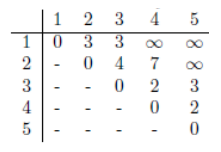
\includegraphics{figures/problema1/matriz_costes.png}
    \caption{matriz de costes}
    \label{fig:enter-label}
\end{figure}
\section{Solución: Diseño de componentes y del algoritmo}


\subsection{Resolución del problema por etapas}
En cada etapa se seleccionaría ir o no a una aldea próxima. 
Supondremos que las aldeas están ordenadas de menor a mayor coste para asegurar una solución óptima factible desde las etapas más tempranas.

\subsection{Ecuación recurrente}
Nuestra ecuación de recurrencia consta de el calculo del mínimo coste de entre  ir directamente de la aldea i hasta la aldea j  o tomar otras canoas en otras aldeas anteriores.
Siendo Coste(i,j) el coste directo de ir de i a j en canoa y MIN(i,k)+MIN(k,j)  siendo el calculo de otro camino para ir desde la aldea i hasta la aldea j alquilando otra canoa en algún pueblo anterior.
A esta ecuación de recurrencia se le añaden las restricciones de que no podemos cambiar de canoas en aldeas mas arriba del río debido a la corriente. Esto lo reflejamos con k>i y k<j. k siendo una aldea intermedia de nuestro recorrido.

\[ MIN(i, j) = min
  \left \{
    \begin{aligned}
      Coste (i, j)\\
      MIN(i, k) + MIN(k, j)    & \text{si } i<k<j
    \end{aligned}
  \right .
\]

 
\subsection{Valor objetivo}
Se desea conocer el valor OPT(i,j), el mínimo coste para realizar un viaje desde la primera aldea hasta la aldea a la que se desea llegar. 

\subsection{Verificación del cumplimiento del P.O.B}
Para demostrar que se aplica el principio de optimalidad de Bellman tenemos que demostrar que la solución óptima se consigue a partir de las soluciones óptimas los subproblemas que componen a nuestro problema. En este caso estos subproblemas son los costes mínimos de viajar desde una aldea (i) hasta otra aldea (j) para diferentes valores de i.
En este caso se cumple debido a que nuestra ecuación de recurrencia siempre va escogiendo el mínimo coste no es posible que exista una forma alternativa para ir desde la aldea i hasta la aldea j con un menor coste.

\subsection{Diseño de la memoria} 
Para el diseño de la memoria, decidimos usar una matriz en la que almacenar los costes mínimos ya calculados para ir de una aldea \textit{i} a otra \textit{j}. 
Para ello, usamos una matriz en la que se irán almacenando los valores de costes calculados. Cuando esta matriz este completa (solo la mitad superior, debido a la naturaleza del problema) se nos quedara la solución en la primera fila en forma de costes.
Cuando esto ocurra pasaremos estos costes a nuestro camino ya con el numero correspondiente a cada aldea por las que tendremos que pasar en forma de secuencia.
\subsection{Diseño del algoritmo de cálculo de coste óptimo}
\begin{lstlisting}
    calcviajeopt( matriz rio, matriz opt, salida, destino){
        para i=destino-1 hasta salida{
            para j=destino hasta i {
                opt[i][j]=rio[i][j] + min(fila j de opt)
            }
        }
        Devolver min(opt[salida])
    }
\end{lstlisting}
Para la resolución de este problema, hemos simplificado la idea de programación dinámica agregando las restricciones que nos imponía el enunciado. De esta forma, y como se puede observar en el pseudocódigo anterior, únicamente rellenaremos la mitad de la tabla(debido a la imposibilidad de acceder a una canoa que hayamos dejado atrás). Así, rellenaremos cada casilla de nuestra tabla con la distancia desde la aldea de la que procedamos hasta la que estemos comprobando en el momento, sumada a la mínima distancia posible desde esta última aldea a nuestro destino final.
Una vez la tabla se encuentre rellena, nuestra solución final corresponderá al mínimo almacenado en la fila correspondiente al punto de salida de nuestra tabla.


\subsection{Diseño del algoritmo de recuperación de la solución}
\begin{lstlisting}
    camino recuperarsol(matriz rio, matriz opt, salida, destino){
        camino = vacio
        
        minimo=min(opt[salida])
        camino += salida
        camino += minimo
        
        mientras minimo sea distinto de destino{
            minimo=min(opt[minimo])
            camino + =  minimo
        }
        Devolver camino
    }
\end{lstlisting}
Conociendo la tabla rellenada tras la ejecución del algoritmo anterior, buscaremos conocer en que aldeas hemos parado para obtener el camino a recorrer. Por ello, buscaremos el mínimo de nuestra fila de salida, añadiendo a nuestro camino tanto nuestra aldea de partida como la aldea en la que realizaremos la primera parada(correspondiente al mínimo).
A continuación realizaremos esto sucesivamente hasta llegar al destino, tomando como partida la aldea en la que hayamos realizado la parada y añadiendo a la solución únicamente las siguientes en las que vayamos a parar.

% \chapter{Problema 2}

\section{Descripción del problema}

Una empresa realiza planificaciones de viajes aéreos entre \textit{n} ciudades. Para ir de una ciudad \textit{i} a una ciudad \textit{j} puede ser necesario coger varios vuelos distintos. El tiempo de un vuelo directo de \textit{i} a \textit{j} será (si existe) \textit{T(i,j)} (que puede ser distinto de \textit{T(j,i}). Hay que tener en cuenta que si cogemos un vuelo de \textit{i} a \textit{k} y después otro de \textit{k} a \textit{j}, será necesario esperar un tiempo de \textit{escala} adicional \textit{E(k)} en el aeropuerto de \textit{k}, con lo que el tiempo de ese viaje de \textit{i} a \textit{j} será de \textit{T(i,k) + T(k,j) + E(k)}.

Se desea conocer la forma de volar desde cualquier ciudad \textit{i} hasta cualquier otra \textit{j} en el menor tiempo posible. Diseñad e implementad un algoritmo de Programación dinámica que resuelva este problema. Aplicadlo para resolver el problema, para n=4, cuya matriz de tiempos es la siguiente, suponiendo que \textit{E(k)} = 1 para cualquier valor de k.

\begin{figure}
    \centering
    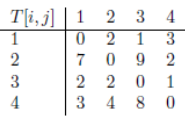
\includegraphics[width=0.5\linewidth]{figures/problema2/tabla2.png}
\end{figure}

\section{Solución: Diseño de componentes y del algoritmo}


\subsection{Resolución del problema por etapas}

La forma de resolver cada etapa será elegir si tardamos menos tiempo tomando un vuelo directo al destino final o haciendo escala en otro aeropuerto y luego tomar un vuelo al destino final. En esta comparación habrá que tener en cuenta la posibilidad de hacer escala en cualquiera de los 2 aeropuertos restantes que tenemos, ya que no tendrá sentido hacer escala en el aeropuerto del que salimos o al que pretendemos llegar ya que realmente no estaríamos haciendo escala alguna, tan solo sumaríamos el coste de estar haciendo una escala que no existe. 

Realmente lo que usaremos será el Algoritmo de Floyd (con alguna pequeña modificación para que sea más entendible), pues el problema se puede ver como calcular el camino más corto que une un par de vértices de un grafo.

\subsection{Ecuación recurrente}

La ecuación recurrente constará, por tanto, de calcular el mínimo de entre tomar un vuelo directo o hacer escala en un aeropuerto distinto tanto al de origen como el de llegada y luego ir al destino final.
\[
tiempo\_minimo(i, j) =  \min \begin{cases} 
tiempo (i, j) \\
tiempo\_min(i, k) + tiempo\_min(k, j) + E(k) para todo k!=i,j\\
\end{cases}
\]

El caso base del que partimos es la matriz de tiempos inicial, es decir, \(tiempo\_min_{0}(i,j) = tiempo(i,j)\)

Realmente es hacer un mínimo entre 3 cosas, el coste de ir directo y el coste de hacer escala en los otros 2 aeropuertos restantes que no sean ni el punto de partida ni el punto de llegada, ya que entonces no estaríamos haciendo escala alguna, más el coste de hacer escala y luego hacer otro vuelo al destino final.

\subsection{Valor objetivo}

Se desea conocer el valor \textit{tiempo\_minimo(i,j)}, el tiempo mínimo que se puede tardar en ir de un aeropuerto \textit{i} a otro aeropuerto \textit{j} dados una serie de duraciones de vuelos entre diversos aeropuertos y el coste \textit{E(k)} de hacer escalas.

\subsection{Verificación del cumplimiento del P.O.B}

El principio de optimalidad de Bellman se verifica cuando toda solución óptima está compuesta por soluciones óptimas de sus subproblemas. En nuestro caso, las soluciones óptimas de los subproblemas se obtienen al calcular el tiempo mínimo que se tarda en ir entre cada par de nodos (al calcularse como el mínimo de todas las posibilidades para ir a ese punto ya sea de forma directa o haciendo escala, podemos considerar que esa solución será óptima). De esta forma, cuando tengamos que construir una solución óptima final para un origen y destino concretos, lo estaremos haciendo a partir de soluciones óptimas de los subproblemas ya calculados. Al asegurar que los viajes más cortos encontrados entre todos los aeropuertos son compuestos de subviajes que también son las más cortos posibles, podemos concluir que se cumple el principio de optimalidad de Bellman.

\subsection{Diseño de la memoria}

Para el diseño de la memoria, decidimos usar una matriz en la que almacenar los tiempos mínimos ya calculados para ir de un aeropuerto \textit{i} a otro aeropuerto \textit{j}. Para futuras ejecuciones del algoritmo, antes de usarlo bastará con comprobar si el valor en la casilla es válido (distinto de -1) o no para ver si es necesario ejecutar el algoritmo o simplemente basta con recuperar el valor deseado porque se haya calculado previamente.

Para ello, usamos una matriz en la que se irán almacenando los valores de tiempos mínimos calculados, la cual comenzará inicializada como la matriz de tiempos originales y sobre la cual se aplicará el Algoritmo de Floyd para hallar el camino más corto que une un par de vértices de un grafo, es decir, dos aeropuertos.

También iremos rellenando una matriz de antecesores, la cual nos será útil para realizar la recuperación de la solución, por lo que será explicado más tarde.

\subsection{Diseño del algoritmo de cálculo de coste óptimo}

Como ya hemos explicado anteriormente, tras aplicar el algoritmo de Floyd bastará con consultar la posición indicada de la matriz para saber cuál es el tiempo mínimo que se puede tardar en ir de un aeropuerto a otro, siendo el coste óptimo el mínimo entre tomar un vuelo directo y hacer escala en otros aeropuertos.

Con este diseño, construimos el algoritmo de Programación Dinámica como sigue:

\begin{lstlisting}
origen y destino -> aeropuertos de origen y destino
tiempos -> matriz de tiempos de vuelo directos entre aeropuertos
tiempos_min -> matriz de tiempos mínimos calculados
antecesores -> matriz donde almacenamos de qué aeropuerto venimos en cada iteracion del bucle. Inicialmente tendra el origen de los vuelos directos ya que no se consideran escalas.

tiempo_min (origen, destino, tiempos[nxn], tiempos_min[nxn], antecesores[nxn]){

    tiempos_min = tiempos
    Para cada k hasta n
        Para cada i hasta n
            Para cada j hasta n
                si k!=i,j // si realmente podemos hacer una escala
                    tiempos_min (i,j) = min (tiempos_min(i,j), tiempos_min(i,k) + tiempos_min(k,j) + 1)
                    si tiempos_min (i,j) == tiempos_min(i,j), tiempos_min(i,k) + tiempos_min(k,j) + 1 // si he hecho escala, modifico la matriz de antecesores para saber dónde he hecho escala
                        antecesores(i,j) = k
                    
    devolver tiempos_min(origen, destino)                   
}

\end{lstlisting}

\subsection{Diseño del algoritmo de recuperación de la solución}

Para recuperar la solución y ver en qué aeropuertos hemos hecho escala, bastará con ir rellenando una matriz de antecesores al mismo tiempo que calculamos las distancias mínimas. De esta forma, tras haber ejecutado el algoritmo bastará con ir consultando la tabla de adyacencia e ir consultando los valores de la misma hasta dar con una posición en el que ya se haya llegado al origen del viaje.

Inicialmente la tabla de antecesores almacenará el valor del aeropuerto desde el cual se hace el vuelo directo, ya que los tiempos mínimos comenzarán siendo los que se tardan en ir con vuelos directos y aún no se han considerado las escalas.

Al calcular los tiempos mínimos, si se ha hecho una escala se modifica la matriz de antecesores y se pone como valor el aeropuerto en el que se hace escala para poder llegar hasta el destino final. De esta forma, para recuperar el conjunto de aeropuertos que hay que recorrer para ir de un origen a un destino tendremos que ir moviéndonos por la matriz de antecesores comenzando por la casilla final a la que queremos ir hasta que lleguemos al punto en el que el antecesor sera el origen del que partimos. Iremos almacenando en el camino los aeropuertos que vamos visitando, aunque los almacenaremos en orden inverso y luego le tendremos que dar la vuelta para obtener la ruta realizada.

Con este diseño, construimos el algoritmo de recuperación de la solución como sigue:

\begin{lstlisting}
sol -> conjunto de aeropuertos visitados

recuperar_sol(origen, destino, antecesores[nxn]{
    sol = conjunto vacio
    sol = sol U {antecesores(origen, destino)} // Incluimos el aeropuerto final
    col = destino
    
    hacer{
        anterior = antecesores (origen,col)
        sol = sol U {anterior} // Aniadimos de donde venimos
        col = anterior // Para ver como hemos llegado hasta ahi la siguiente iteración
    } mientras que anterior != origen

    // Dar la vuelta a sol para tener ordenados los aeropuertos que visitamos

    devolver sol
}
\end{lstlisting}



% \chapter{Problema 3}

\section{Descripción del problema}
Un videojuego se juega por turnos y se representa en un mapa cuadriculado bidimensional
de f filas y c columnas. El jugador siempre entra al mapa por la esquina superior derecha,
y sale por la esquina inferior izquierda. En cada turno, los posibles movimientos del
jugador son: ir 1 casilla a la izquierda, ir 1 casilla abajo, o moverse 1 posición a la casilla
inferior izquierda. Cada casilla del mapa puede estar vacía, contener un muro, o contener
una bolsa de oro. Todas las casillas son transitables salvo las que tienen muros. El objetivo
consiste en llegar a la salida pudiendo recoger tanto oro como sea posible (pasar por tantas
casillas que contengan una bolsa como se pueda). En el ejemplo siguiente, el jugador
puede conseguir un máximo de 3 bolsas de oro con los movimientos permitidos.

\begin{figure}[h]
    \centering
    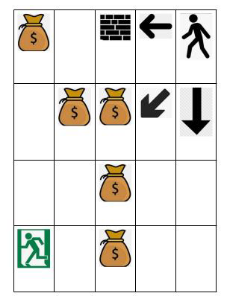
\includegraphics[width=0.4\linewidth]{figures//problema3/imagen.png}
    \label{fig:enter-label}
\end{figure}

\section{Solución: Diseño de componentes y del algoritmo}


\subsection{Resolución del problema por etapas}

Este problema puede resolverse mediante etapas. En cada etapa podemos barajar que posibilidad nos sale más rentable acorde a nuestros objetivos. Como nuestros objetivos son maximizar la cantidad de oro que vamos recogiendo en función de las casillas por las que pasamos, debemos de escoger aquellas posiciones, que en cómputo total, al salir del mapa del juego consigamos la máxima cantidad de bolsas de oro. Cabe destacar que para las explicaciones que vamos a realizar a continuación vamos a pensar que la representación del mapa va a corresponder con una matriz.

\subsection{Ecuación recurrente}

La solución depende de las etapas (a que posición debo de mover el personaje del videojuego para obtener la mayor cantidad de oro). Vamos a denotar como $T(i,j)$ el máximo número de bolsas de oro que se puede conseguir al llegar a la casilla $(i,j)$. Como sabemos \textit{i} y \textit{j} corresponde con las posiciones dentro de nuestro mapa del videojuego.

Debemos de considerar el tipo de casilla, ya que puede ser casilla con muro, sin muro, y dentro de sin muro que haya oro o no. Lo que haremos será denotar a las casillas con un valor negativo muy grande, es decir, casillas = \(-\infty\). Para inicializar toda la matriz, y ya mediante el algoritmo de programación dinámica vamos a ir resolviendo el problema y devolver una matriz final T, la cual explicaremos a continuación. 
Por lo que podemos afirmar que si la casilla \textit{(i,j)} tiene un muro $T(i,j)$ = \(-\infty\). Esto lo ampliamos a que valdrá $T(i,j)$ = \(-\infty\) cuando, en general, la casilla sea no transitable. También el valor puede llegar a ser no accesible debido a la propagación de la innaccibilidad. Al calcular los valores de \textit{T(i)(j)}, si todos los caminos posibles hacia una celda provienen de celdas inaccesibles (es decir, que contienen \textit{INT\_MIN}), entonces esa celda también será inaccesible. De esta manera, la inaccessibilidad se propaga correctamente a través de la matriz. Esta representación ayuda a asegurar que las celdas inalcanzables no se utilicen en cálculos posteriores.

En el caso de que no sea un muro, podemos establecer el valor de $T(i,j)$ en función de que si hay oro o no en la casilla. Así que podemos expresar $T(i,j)$ cuando no hay un muro de la siguiente manera:

\[T(i,j) = max \{T(i-1,j-1),T(i-1,j),T(i,j-1) + Oro(i,j)\} \]

Cabe destacar que va a variar en función de la posición en la que nos encontremos, ya que en el caso de que \textit{(i,j)} sea \textit{(0,0)} no se pueden acceder a diversas posiciones. La función \textit{Oro(i,j)} devuelve \textit{1} en el caso de que si haya oro en la casilla \textit{(i,j)} y \textit{0} en caso contrario.

En base a este planteamiento, podemos establecer que nuestra ecuación de recurrencia sería:

\[
T(i, j)  \begin{cases} 
T(i,j) = -\infty\ \text{   si hay un muro en (i,j) o es una casilla no transitable} \\
T(i,j) = max \{T(i-1,j-1),T(i-1,j),T(i,j-1) + Oro(i,j)\} \text{  si no hay muro en (i,j)}
\end{cases}
\]

Los casos base para esta ecuación serían: 

\begin{itemize}
    \item Si nos encontramos en la casilla inicial estamos en $T(0,0) = Oro (0,0)$. El valor depende si hay oro o no en la casilla inicial.
    \item Si nos encontramos una casilla se encuentra fuera del mapa o que posee un muro, se considera una casilla no transitable.
\end{itemize}

\subsection{Valor objetivo}

Se desea conocer $T(i,j)$, el valor máximo de bolsas de oro que se pueden conseguir transitando desde la casilla \textit{(0,0)} hasta la casilla (n-1,m-1) teniendo la posibilidad de moverse a las casillas \textit{(i-1,j-1), (i-1,j) y (i,j-1)}, podemos acceder a esas posiciones siempre y cuando \( i \in {0..n-1} \) y \( j \in {0..m-1} \)

\subsection{Verificación del cumplimiento del P.O.B}
En este caso siempre estamos calculando la solución óptima ya que la optimalidad de la casilla de \textit{(i,j)} se ha calculado en base a otros casos que a su vez también son óptimos, por lo que podemos concluir que también es óptimo. Básicamente, Cualquier solución óptima debe estar formada por subsoluciones óptimas. En este caso se cumple, dado que \textit{T(i,j)}, que asumimos óptimo, podrá tener valores \textit{T(i-1,j-1), T(i-1,j) o T(i,j-1)}. Estos valores también son óptimos, dado que la ecuación recurrente siempre va escogiendo el máximo entre los valores mencionados anteriormente. No es posible que exista un valor mayor que el máximo entre los valores para \textit{T(i,j).}

\subsection{Diseño de la memoria}
\begin{itemize}
    \item Para resolver el problema, usaremos una matriz, por lo que, \textit{T (i,j)} se representará como una matriz.
    \item Esta matriz tendrá n filas y m columnas, que estarán asociadas a el lugar correspondiente dentro del mapa. Únicamente, podrán optar por valores entre {0...n-1}.
    \item Cada celda de la matriz \textit{T(i,j)} contendrá el máximo valor de bolsas de oro que se pueden obtener hasta llegar a la casilla \textit{(i,j)} del mapa teniendo en cuenta los movimientos disponibles que se exponen en el problema.
    \item La manera en la que se va a ir rellenando la memoria (matriz) corresponde con ir asignando el correspondiente valor \textit{T(i,j)} a cada casilla de la matriz.
\end{itemize}

\subsection{Diseño del algoritmo de cálculo de coste óptimo}

Con este diseño, construimos el algoritmo de Programación Dinámica como sigue:

\begin{lstlisting}
    ALGORITMO T, V = Max_oro(mapa, n, m)
    T <- matriz de n filas y m columnas indexadas {0...n-1} y {0...m-1}
    
    Para cada posicion de la matriz (i, j) con \( i,j \in {0..n-1} \) hacer:
        T(i, j) = 0
    
    T(0, 0) = Oro(0, 0)  # Inicializamos la primera casilla
    
    Para cada fila i en {0...n-1}, hacer:
        Para cada columna j en {0...m-1}, hacer:
            Si mapa[i][j] es muro, entonces:
                T(i, j) = -infintio o INT_MIN
            Sino:
                oro = Oro(i, j)
                Si i > 0 y j > 0, entonces:
                    T(i, j) = max(T(i, j), T(i-1, j-1) + oro)
                Si i > 0, entonces:
                    T(i, j) = max(T(i, j), T(i-1, j) + oro)
                Si j > 0, entonces:
                    T(i, j) = max(T(i, j), T(i, j-1) + oro)
    
    V <- T(n-1, m-1) //valor maximo de bolsas de oro
    Devolver T, V (siendo V el valor maximo de bolsas de oro)

FUNCION Oro(i, j)
    Si mapa[i][j] == 'O', entonces:
        devolver 1
    Sino:
        devolver 0

        
\end{lstlisting}

Vamos a explicar en detalle el algoritmo del cálculo del coste óptimo. En este creamos T que es la matriz, la cual definimos en base a un número de filas y de columnas determinadas. Posteriormente, inicializamos todas las posiciones de la matriz en 0, es decir, inicializamos la matriz. Inicializamos la casilla inicial. Luego recorremos la matriz por filas y columnas y si vemos que en la posición (i,j) de la matriz hay un muro, le asignamos el valor de \(-\infty\), si no hay muro entonces vemos si podemos comparar con casillas anteriores y con ayuda de la ecuación de recurrencia, calculamos el valor de bolsas de oro para esa casilla, teniendo en cuenta las casillas anteriores. Finalmente almacenamos el valor de bolsas máximas de oro que hay en la última casilla de la matriz, es decir, en la casilla \textit{(n-1,m-1)} y T que es la matriz resultante.

\subsection{Diseño del algoritmo de recuperación de la solución}
\begin{lstlisting}
    ALGORITMO ruta = Recuperar_solucion(T, mapa, n, m)
    ruta <- lista vacia
    i <- n-1
    j <- m-1
    
    Mientras i > 0 o j > 0 hacer:
        anadir (i, j) a ruta
        Si i > 0 y j > 0 y T(i, j) == T(i-1, j-1) + Oro(i, j), entonces:
            i <- i-1
            j <- j-1
        Sino si i > 0 y T(i, j) == T(i-1, j) + Oro(i, j), entonces:
            i <- i-1
        Sino si j > 0 y T(i, j) == T(i, j-1) + Oro(i, j), entonces:
            j <- j-1
    
    anadir (0, 0) a ruta
    invertir ruta  # La ruta se construyo desde el final al inicio
    
    Devolver ruta

FUNCION Oro(i, j)
    Si mapa[i][j] = 'O', entonces: 
        devolver 1
    Sino:
        devolver 0

\end{lstlisting}

Vamos a explicar el diseño del algoritmo de recuperación de la solución. En este caso creamos una lista vacía donde vamos a almacenar la ruta del algoritmo, y vamos
a comenzar por la última posición de la matriz. De manera que mientras haya posiciones por las que volver a la posición inicial vamos a ir comparando si la cantidad de oro es la misma, en el caso de que si quiere decir que esa posición de la matriz es una de las posiciones por la cual podemos pasar desde el inicio hasta el final para obtener la máxima cantidad de bolsas de oro posible. Añadimos esa posición a nuestra lista y finalmente añadimos el inicio para tener la lista completa. Invertimos la ruta para tenerla en el orden correcto y la devolvemos. La notación \textit{'O' y 'M'}, hace referencia a si hay oro o si hay un muro, respectivamente.

La función Oro, únicamente comprueba si la posición (i,j) de la matriz esta etiquetada con \textit{'O'} (hay oro), si lo esta devuelve uno como respuesta de que hay una bolsa de oro, y en caso contrario 0.




    

% \chapter{Problema 4}

\section{Descripción del problema}
El problema consiste en encontrar el camino de menor coste al ascender la "Pixel Mountain". La montaña se representa como una matriz de costes, donde cada elemento $(i, j)$ de la matriz indica el coste de posicionarse en ese punto. El objetivo es encontrar el camino desde la base (fila 0) hasta la cumbre (última fila) con el menor coste posible. Se permiten movimientos hacia arriba, arriba a la izquierda, y arriba a la derecha. Formalmente, queremos minimizar el coste total al llegar a cualquier posición en la cumbre $(f-1, j)$.

\section{Solución: Diseño de componentes y del algoritmo}

\subsection{Resolución del problema por etapas}
Para resolver este problema, utilizamos una técnica de programación dinámica. La idea es construir una tabla $T$ donde cada entrada $T(i, j)$ represente el coste mínimo para alcanzar la posición $(i, j)$ de la montaña. Consideremos la siguiente matriz de costes como ejemplo:

\[
\text{Montaña} = \begin{bmatrix}
4 & 7 & 8 & 6 & 4 \\
6 & 7 & 3 & 9 & 2 \\
3 & 8 & 1 & 2 & 4 \\
7 & 1 & 7 & 3 & 7 \\
2 & 9 & 8 & 9 & 3 \\
\end{bmatrix}
\]

La matriz $T$ se llenará de la siguiente manera:

\[
T(i, j) = \text{coste}(i, j) + \min \begin{cases} 
T(i-1, j) \\
T(i-1, j-1) & \text{si } j > 0 \\
T(i-1, j+1) & \text{si } j < \text{número de columnas} - 1 
\end{cases}
\]

Comenzamos inicializando la primera fila de $T$ con los valores de la primera fila de la matriz de costes, ya que esas son las posiciones de partida.

\[
T(0, j) = \text{Montaña}(0, j)
\]

Para las demás filas, aplicamos la ecuación recurrente para llenar la tabla:

\[
T = \begin{bmatrix}
4 & 7 & 8 & 6 & 4 \\
10 & 11 & 7 & 15 & 6 \\
13 & 15 & 8 & 9 & 10 \\
20 & 9 & 15 & 12 & 16 \\
11 & 18 & 17 & 21 & 15 \\
\end{bmatrix}
\]

Finalmente, el coste mínimo para alcanzar la cumbre de la montaña es el valor mínimo en la última fila de $T$:

\[
V = \min \{ T(f-1, j) \mid 0 \leq j < \text{número de columnas} \} = 11
\]

Para recuperar el camino de menor coste, partimos desde la posición en la última fila de $T$ que contiene el valor mínimo y rastreamos hacia atrás utilizando las posiciones anteriores de donde provino el coste mínimo. Esto nos permite reconstruir el camino óptimo.
\subsection{Ecuación recurrente}
La ecuación recurrente para calcular el coste mínimo para cada posición se define como:
\[
T(i, j) = \text{coste}(i, j) + \min \begin{cases} 
T(i-1, j) \\
T(i-1, j-1) & \text{si } j > 0 \\
T(i-1, j+1) & \text{si } j < \text{número de columnas} - 1 
\end{cases}
\]

Aquí, $\text{coste}(i, j)$ es el coste asociado a la posición $(i, j)$. La función $\min$ selecciona el coste mínimo entre las posiciones desde las que se puede llegar a $(i, j)$, es decir, desde $(i-1, j)$, $(i-1, j-1)$ si $j > 0$, y $(i-1, j+1)$ si $j < \text{número de columnas} - 1$.

\subsection{Valor objetivo}
El valor objetivo es el coste mínimo para alcanzar cualquier posición en la última fila (cumbre) de la matriz. Formalmente, esto se expresa como:
\[
V = \min \{ T(f-1, j) \mid 0 \leq j < \text{número de columnas} \}
\]
donde $f$ es el número de filas de la matriz.

\subsection{Verificación del cumplimiento del P.O.B}

El Principio de Optimalidad de Bellman (P.O.B.) establece que una solución óptima de un problema de optimización se puede obtener a partir de las soluciones óptimas de sus subproblemas. En nuestro contexto, esto significa que el coste mínimo para llegar a la posición $(i, j)$ en la montaña debe ser calculado usando las soluciones óptimas de las posiciones anteriores $(i-1, j)$, $(i-1, j-1)$ y $(i-1, j+1)$. 

Para verificar que nuestra ecuación recurrente cumple con el P.O.B., consideremos que estamos en la posición $(i, j)$:

\[
T(i, j) = \text{coste}(i, j) + \min \begin{cases} 
T(i-1, j) \\
T(i-1, j-1) & \text{si } j > 0 \\
T(i-1, j+1) & \text{si } j < \text{número de columnas} - 1 
\end{cases}
\]

Cada subproblema $T(i-1, j)$, $T(i-1, j-1)$ y $T(i-1, j+1)$ representa el coste mínimo para alcanzar las posiciones inmediatas anteriores desde donde se puede llegar a $(i, j)$. Al tomar el mínimo de estos subproblemas y sumarle el coste de la posición actual $\text{coste}(i, j)$, garantizamos que estamos construyendo la solución óptima de forma inductiva, basada en soluciones óptimas de subproblemas más pequeños. Por lo tanto, nuestra solución cumple con el Principio de Optimalidad de Bellman.


\subsection{Diseño de la memoria}
Con este diseño, construimos el algoritmo de Programación Dinámica como sigue:


\subsection{Diseño del algoritmo de cálculo de coste óptimo}
\begin{lstlisting}
Algoritmo CalcularCosteMinimo(Montana)
    f = numero de filas en Montana
    c = numero de columnas en Montana
    T = matriz de tamaño f x c, inicializada con infinito

    Para j desde 0 hasta c-1 hacer
        T(0, j) = Montana(0, j)

    Para i desde 1 hasta f-1 hacer
        Para j desde 0 hasta c-1 hacer
            T(i, j) = Montana(i, j) + T(i-1, j)
            Si j > 0 entonces
                T(i, j) = min(T(i, j), Montana(i, j) + T(i-1, j-1))
            Fin Si
            Si j < c-1 entonces
                T(i, j) = min(T(i, j), Montana(i, j) + T(i-1, j+1))
            Fin Si
        Fin Para
    Fin Para

    V =  min(T(f-1))
    
    devolver T, V
Fin Algoritmo
\end{lstlisting}

En este pseudocódigo:
\begin{itemize}
    \item Inicializamos la primera fila de la matriz $T$ con los valores de coste de la primera fila de la montaña.
    \item Llenamos la matriz $T$ de manera iterativa usando la ecuación recurrente.
    \item Finalmente, encontramos el valor objetivo $V$, que es el mínimo valor en la última fila de $T$.
\end{itemize}

\subsection{Diseño del algoritmo de recuperación de la solución}
Para recuperar la solución (el camino de menor coste), seguimos el rastro desde la cumbre hasta la base utilizando la tabla $T$:

\newpage
\begin{lstlisting}
Algoritmo RecuperarSolucion(T, Montana)
    f = numero de filas en Montana
    c = numero de columnas en Montana
    Solucion = lista vacia

    j = Indice de la columna con el valor minimo en T(f-1, :)

    Para i desde f-1 hasta 0 hacer
        anadir (i, j) a Solucion
        Si i > 0 entonces
            Si j > 0 y T(i-1, j-1) == T(i, j) - Montana(i, j) entonces
                j = j - 1
            Sino Si j < c-1 y T(i-1, j+1) == T(i, j) - Montana(i, j) entonces
                j = j + 1
            Fin Si
        Fin Si
    Fin Para

    invertir Solucion
    devolver Solucion
Fin Algoritmo
\end{lstlisting}

En este pseudocódigo:
\begin{itemize}
    \item Iniciamos en la última fila de $T$ y encontramos la columna $j$ con el valor mínimo.
    \item Rastreamos el camino desde la cumbre hasta la base, verificando de dónde provino el mínimo coste en cada paso.
    \item Almacenamos cada paso en la lista `Solucion`.
    \item Invertimos la lista `Solucion` para obtener el camino desde la base hasta la cumbre.
\end{itemize}

\input{../Practica-1/Capitulos/p1}
\input{../Practica-1/Capitulos/p2}
\input{../Practica-1/Capitulos/p3}
\input{../Practica-1/Capitulos/p4}
\input{../Practica-1/Capitulos/p5}

% ----------------------- %
% BIBLIOGRAFÍA
% ----------------------- %

% Estilo de cita.
\bibliographystyle{apa-good}
%\renewcommand\bibname{Reference}

%[citestyle=numeric]

%\renewcommand\bibname{Bibliografía}
%

% Añadimos la bibliografía al índice
\phantomsection
\end{document}
